
\section{Processing system}
\label{sec:design-components}

As discussed in the previous chapter, the processing system of the library relies on the components.
The core of the library is responsible for just creating the component graph.
The processing of an \lsystem and production of results is fully under the control of the component graph.
This gives absolute freedom to the user in implementing the process system.

However it is hard to design and implement the whole \lsystem processing system from scratch.
The library contains a rich set of predefined components from which can be assembled many different component graphs.
The predefined components have a general interface which allows the user to reuse or extend them in order to add new functionality with a minimum of effort.


\subsection{Basic component system}

The component system designed in this section is primarily used for processing \lsystems to produce 2D and 3D graphics in the web interface.
However, the component system is designed to be extensible to any output type.

\lsystems are generally processed in two phases.
The first phase is rewriting where the axiom (the initial string of symbols) is rewritten by the rewrite rules, and the second phase is interpreting the resulting string of symbols.
This can be done with two components, the Rewriter -- which is responsible for rewriting the \lsystem to a given iteration -- and the Interpreter -- which is responsible for interpreting symbols and producing output (Fig. \ref{fig:simpleSystem}).

\begin{figure}[h!]
	\centering
	\begin{tikzpicture}[->,auto,node distance=3cm,>=latex,shorten >=2pt]
		\node (in) [coord] {};
		\node (rw) [block, right of=in] {Rewriter};
		\node (int) [block, right=1cm of rw] {Interpreter};
		\node (out) [coord, right of=int] {};
		
		\draw (in) -- node {input} (rw);
		\draw (rw) -- (int);
		\draw (int) -- node {output} (out);
	\end{tikzpicture}
	\caption{Simple \lsystem processing system}
	\label{fig:simpleSystem}
\end{figure}

However the components in the system in \autoref{fig:simpleSystem} have too many tasks to do, and thus they will be complicated to implement and hard to extend and test.

The system in \autoref{fig:advancedSystem} was created by a subdivision of the previous system.
The Rewriter component was split to the Rewriter and the Iterator.
The (new) Rewriter will just do the rewriting of some given symbols and the Iterator will control the iterating of the \lsystem (repetitive rewriting).
The Interpreter component was split to the Interpreter and the Renderer.
The (new) Interpreter will handle the interpreting of symbols: which means keep position of the virtual "turtle" in space, saving and loading of states, etc.
The Renderer will just produce the output.
If we need to create a different output type we only have to implement the new renderer component and the rest of the system will remain unchanged.

\begin{figure}[h!]
	\centering
	\begin{tikzpicture}[->,auto,node distance=3cm,>=latex,shorten >=2pt]
		\node (rw) [block] {Rewriter};
		\node (iter) [block, right of=rw] {Iterator};
		\node (in) [coord, above of=iter, node distance=15mm] {};
		\node (inter) [block, right of=iter] {Interpreter};
		\node (rend) [block, right of=inter] {Renderer};
		\node (out) [coord, right of=rend] {};
		
		\draw (rw) to[bend left=40] (iter);
		\draw (iter) to[bend left=40] (rw);
		\draw (in) -- node {input} (iter);
		\draw (iter) -- (inter);
		\draw (inter) -- (rend);
		\draw (rend) -- node {output} (out);
	\end{tikzpicture}
	\caption{Subdivided \lsystem processing system}
	\label{fig:advancedSystem}
\end{figure}


\subsection{Component system extensions}
\label{sec:caller}

The system in \autoref{fig:callerComponent} can be enhanced even more.
Every component that interprets \lsystem symbols needs to translate symbols to interpretation methods.
The translation can be implemented by every component individually.
However, the translation can be done by a specialized component called the \emph{Interpreter caller}.
This component can be smart enough to explore all the components in the system, find all the interpretation methods of all components and do translation automatically.
This causes an automatic "connection" of all interpreters to the interpreter caller.

More interpreters can be used to advantage: for example, for processing \lsystems which interact with themselves or their Environment \cite{MP96}.
One interpreter actually creates the result model and the second interpreter simulates the environment.

\begin{figure}[h!]
	\centering
	\begin{tikzpicture}[->,auto,node distance=3cm,>=latex,shorten >=2pt]
		\node (iter) [block] {Iterator};
		\node (in) [coord, above of=iter, node distance=15mm] {};
		\node (rw) [block, below of=iter, node distance=20mm] {Rewriter};
		\node (caller) [blockx, right of=iter, node distance=35mm] {Interpreter caller};
		\node (inter) [block, right of=caller, node distance=40mm] {Interpreter};
		\node (env) [block, below of=inter, node distance=20mm] {Environment module};
		\node (rend) [block, right of=inter] {Renderer};
		\node (out) [coord, right of=rend] {};
		
		\draw (rw) to[bend left=40] (iter);
		\draw (iter) to[bend left=40] (rw);
		\draw (in) -- node {input} (iter);
		\draw (iter) -- (caller);
		\draw [dashed] (caller) -- (inter);
		\draw [dashed] (caller) -- (env);
		\draw (inter) -- (rend);
		\draw (env) -- (rw);
		\draw (rend) -- node {output} (out);
	\end{tikzpicture}
	\caption[Automated interpreter caller]{The Interpreter caller which automatically calls interpretation methods of any components}
	\label{fig:callerComponent}
\end{figure}




The next necessary component is called the \emph{Random provider}.
It provides controlled behavior for random number generation as described in \autoref{sec:measuring}.
This component provides a function which returns a random number and it can be called by other components or by the user in the \lsystem definition.
This component is connected to the iterator to correctly the reset random seed at every pass.

The \emph{axiom provider} is the next extending component and it provides the axiom to the Iterator.
The axiom provider is only a "wrapper" around a single symbol property called the axiom.
The Iterator is designed generally to take the axiom from any component implementing \emph{ISymbolProvider} interface so it is possible to connect, for example, another rewriter as the axiom provider (Fig. \ref{fig:inputProvider}).

\begin{figure}[h!]
	\centering
	\begin{tikzpicture}[->,auto,node distance=3cm,>=latex,shorten >=2pt]
		\node (iter) [block] {Iterator};
		\node (rw) [block, left of=iter] {Main rewriter};
		\node (rw2) [blockx, above of=iter, node distance=20mm] {Input rewriter};
		\node (in) [coord, above of=rw2, node distance=15mm] {};
		\node (caller) [block, right of=iter, node distance=35mm] {Interpreter caller};
		\node (inter) [block, above of=caller, node distance=20mm] {Interpreter};
		\node (rend) [block, right of=inter] {Renderer};
		\node (out) [coord, right of=rend] {};
		
		\draw (rw) to[bend left=40] (iter);
		\draw (iter) to[bend left=40] (rw);
		\draw (rw2) -- (iter);
		\draw (in) -- node {input} (rw2);
		\draw (iter) -- (caller);
		\draw [dashed] (caller) -- (inter);
		\draw (inter) -- (rend);
		\draw (rend) -- node {output} (out);
	\end{tikzpicture}
	\caption{Input for the iterator can be supplied by another component}
	\label{fig:inputProvider}
\end{figure}



\subsection{Interpretation of a symbol as another \lsystem}
\label{sec:innerLsystem}

In some situations it can be handy to interpret a symbol as another \lsystem.
The component system of the library is very versatile and it allows the creation of a specialized component which will be responsible for just this feature.

The component is called the \emph{Inner \lsystem processor}.
It is connected to the Interpreter caller and when the caller needs to interpret a symbol as an \lsystem it will call the Inner \lsystem processor to take care of this.
A component graph with the Inner \lsystem processor component is shown in \autoref{fig:innerSystem}.

The Inner \lsystem processor works internally in a similar way to that of the Process manager (see \autoref{sec:inputProcessing}).
For every processed symbol it builds a new components graph for processing the inner \lsystem.
The components graph can be specified by a special process configuration which needs to be defined in the input%
	\footnote{
		The only implementation of the Inner \lsystem processor the \hyperref[Malsys.Processing.Components.Common.LsystemInLsystemProcessor]{\emph{LsystemInLsystemProcessor}} component uses the process configuration called \emph{InnerLsystemConfig} for creating the inner component graph.
		This process configuration must be defined (see the definition in the Standard library \ref{sec:innerLsystemConfig}).}.
The interpreter caller in the inner component graph is automatically connected to all interpreters in the original component graph (see \autoref{sec:caller}), therefore the inner \lsystem is interpreted by the same interpreter as the main \lsystem.
The inner interpreter caller is also connected to the Inner \lsystem processor: thus it is possible to interpret a symbol as another \lsystem even in the inner \lsystem.

The creation of the inner component graph is a relatively complex operation.
The created and used component graphs are cached and reused later which improves the performance.

\begin{figure}[h!]
	\centering
	\begin{tikzpicture}[->,auto,node distance=3cm,>=latex,shorten >=2pt]
		\node (it) [block] {Iterator};
		\node (in) [coord, above of=it, node distance=15mm] {};
		\node (rw) [block, left of=it] {Rewriter};
		\node (caller) [block, right of=it, node distance=35mm] {Interpreter caller};
		\node (inter) [block, above of=caller, node distance=20mm] {Interpreter};
		\node (rend) [block, right of=inter] {Renderer};
		\node (out) [coord, right of=rend] {};
		\node (inner) [blockx, below of=caller, node distance=20mm] {Inner L-system processor};
		\node (innerIt) [blockx, below of=inner, node distance=22mm] {Inner iterator};
		\node (innerRw) [blockx, left of=innerIt, node distance=33mm] {Inner rewriter};
		\node (innerCaller) [blockx, right of=innerIt, node distance=32mm] {Inner caller};
		
		\node (innerArea) [area,fit=(innerIt) (innerRw) (innerCaller), label=above left:Inner component graph] {};
		
		\draw (rw) to[bend left=40] (it);
		\draw (it) to[bend left=40] (rw);
		\draw (in) -- node {input} (it);
		\draw (it) -- (caller);
		\draw (caller) -- (inner);
		\draw [dashed] (caller) -- (inter);
		\draw (inter) -- (rend);
		\draw (rend) -- node {output} (out);
		
		\draw [snakeline] (inner) -- (innerArea);
		\draw (innerRw) to[bend left=20] (innerIt);
		\draw (innerIt) to[bend left=20] (innerRw);
		\draw (innerIt) -- (innerCaller);
		\draw (innerCaller) -- (inner);
		\draw [dashed] (innerCaller) to[bend right] (inter);
	\end{tikzpicture}
	\caption{Component system for interpretation of a symbol as another \lsystem}
	\label{fig:innerSystem}
\end{figure}

The interpretation of symbol as another \lsystem is demonstrated in \autoref{fig:innerLsystem}.
The Pythagoras tree is made of Menger sponges: number of iterations of each Menger sponge depends on its size.
The smallest Menger sponge (zero iteration) has an extra blossom as a demonstration of an interpretation symbol as an \lsystem in the inner \lsystem.
The iteration of the Blossom \lsystem determines the number of leaves and it is randomly selected from 4 to 6.


\begin{figure}[p]
	\centering
	\subfloat[4th iteration]{
\includegraphics[scale=0.3]{Bloom4}}
	\subfloat[5th iteration]{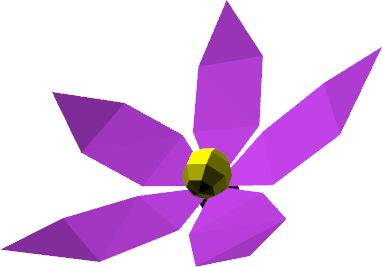
\includegraphics[scale=0.3]{Bloom5}}
	\subfloat[6th iteration]{
\includegraphics[scale=0.3]{Bloom6}}
	\\
	\subfloat[11th iteration of the Pythagoras tree]{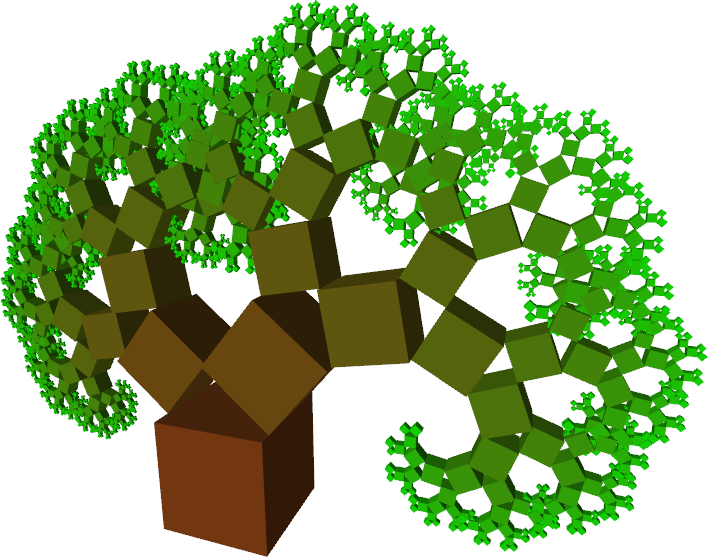
\includegraphics[width=0.55\textwidth]{Pythagoras}} ~
	\subfloat[3rd iteration of the Menger sponge]{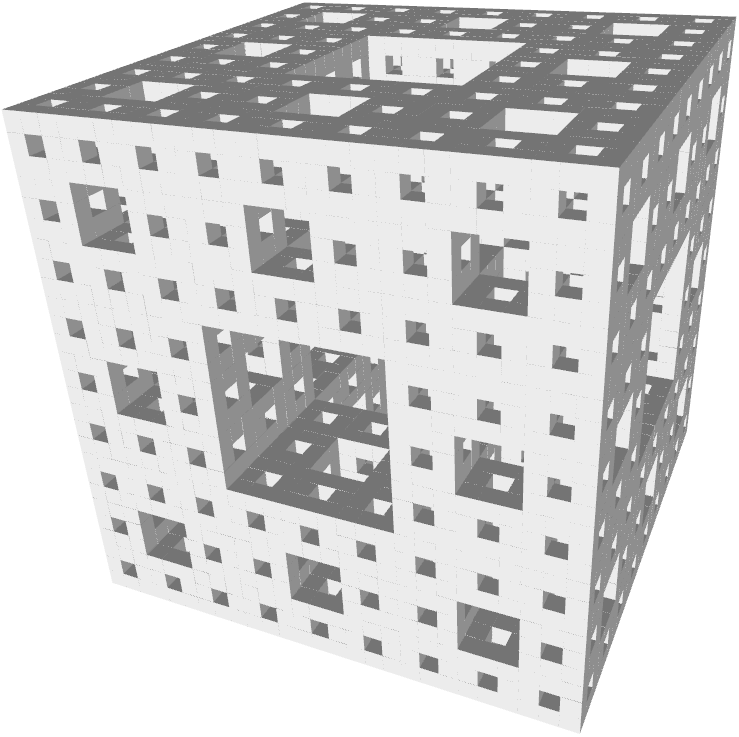
\includegraphics[width=0.40\textwidth]{MengerSponge}}
	\\
	\subfloat[The Pythagoras tree made of the Menger sponges with blossoms at the smallest cubes]{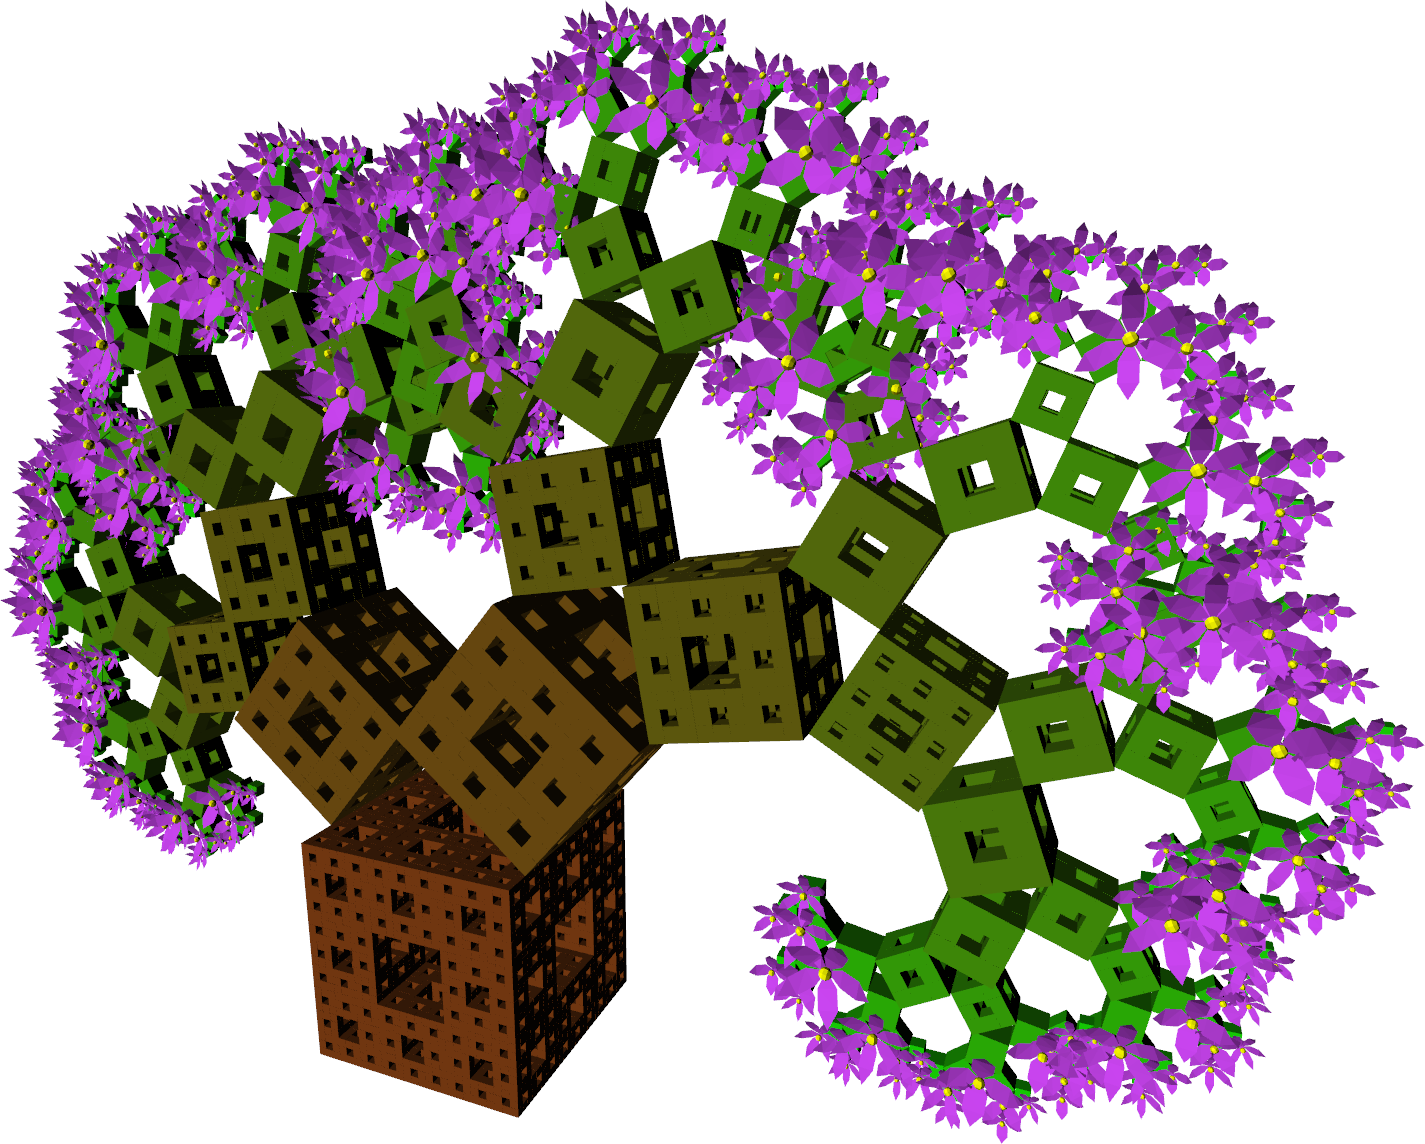
\includegraphics[width=0.9\textwidth]{HybridPythagoras}\label{fig:innerLsystemResult}}
	\caption{Example of interpreting s symbol as another \lsystem}
	\label{fig:innerLsystem}
\end{figure}

\begin{Lsystem}[label=lsys:innerLsystem,caption={Source code of \lsystem (Fig. \ref{fig:innerLsystemResult}) demonstrating use of an interpreting symbol as another \lsystem}]
lsystem HybridPythagorasTree(angle = 50) extends Branches {
	let angleComp = 90 - angle;  // angle complement
	let sinAngle = sin(deg2rad(angle));
	let sinAngleComp = sin(deg2rad(angleComp));
	set iterations = 8;
	set symbols axiom = F(64, 0);
	// interpret E(x) as DrawForward(x, x);  // cube
	@interpret E(x) as lsystem MengerSponge(x);@  // Menger sponge
	interpret m as MoveForward;
	interpret + as Yaw(angle);
	interpret - as Yaw(-angleComp);
	rewrite F(x)
		with left = x * sinAngle, right = x * sinAngleComp
		to E(x) [ + m(left / 2) F(right) ] - m(right / 2) F(left);
}

lsystem MengerSponge(size = 1) extends StdLsystem3D {
	let iters = if(size > 50, 2, if(size > 10, 1, 0));
	let cubeSize = size * (1/3)^iters;
	let renderBlooms = iters == 0;
	// add iteration to render blooms
	let iters = iters + if(renderBlooms, 1, 0);
	set iterations = iters;
	set symbols axiom = F;
	interpret F as DrawForward(cubeSize, cubeSize, #EEEEEE);
	interpret f as MoveForward(cubeSize / 2);
	@interpret B as lsystem Bloom(cubeSize);@  // renderes bloom
	rewrite F where renderBlooms to F [ ^ f B ];
	rewrite F to - f f + & f f ^ F F F +f+f- F F +f+f- F F +f+f- F
		-f+f+f^f F F &f&f^ F F &f&f^ F ^ ^ f f f & + f F F &f&f^ F
		^ ^ f f f & + f F F &f&f^ F ^ ^ f f f & + f F f & f f ^ +
		+ f f - f f f f f;
	rewrite f to f f f;
}

lsystem Bloom(size = 1) extends Polygons {
	let color = #d649ff;
	let leafCount = floor(random(4, 7));
	let angle = 150 / leafCount;
	set iterations = leafCount;
	set symbols axiom = F [ G(size/8) K ] leaf;
	interpret F as DrawForward(size * 0.5, size * 0.2, color);
	interpret G as MoveForward(size * 0.5);
	interpret K as DrawSphere(size / 6, #FFFF00);
	interpret + as Yaw(angle);
	interpret - as Yaw(-angle);
	interpret / as Roll;
	interpret ^ as Pitch(-15);
	rewrite leaf to /(360 / leafCount) [ ^(90) <(color) .
		+ ^ G . - ^ G . - ^ G . + +(180) + G . - ^ G .  > ] leaf;
}

process HybridPythagorasTree with ThreeJsRenderer;
\end{Lsystem}



\subsection{Final component system}

The final component system uses all the described functionality.
The component graph is shown in \autoref{fig:finalSystem}.
Two main \emph{process configurations} defined in the standard library use this scheme, namely the \hyperref[configurationSvgRenderer]{\emph{SvgRenderer}} and the \hyperref[configurationThreeJsRenderer]{\emph{ThreeJsRenderer}}
	(see appendix \ref{sec:stdLibProcessConfigurations}).

\begin{figure}[h!]
	\centering
	\begin{tikzpicture}[->,auto, node distance=3cm,>=latex,shorten >=2pt]
		\node (it) [block] {Iterator};
		\node (in) [block, above of=it, node distance=20mm] {Axiom provider};
		\node (rand) [block, below left of=it, node distance=28.284mm] {Random generator provider};
		\node (rw) [block, left of=it] {Rewriter};
		\node (caller) [block, right of=it, node distance=35mm] {Interpreter caller};
		\node (inter) [block, above of=caller, node distance=20mm] {Interpreter};
		\node (rend) [block, right of=inter] {Renderer};
		\node (out) [coord, right of=rend] {};
		\node (inner) [block, below of=caller, node distance=20mm] {Inner L-system processor};
				
		\draw (rw) to[bend left=40] (it);
		\draw (it) to[bend left=40] (rw);
		\draw (in) -- (it);
		\draw (it) -- (caller);
		\draw (it) -- (rand);
		\draw (caller) -- (inner);
		\draw [dashed] (caller) -- (inter);
		\draw (inter) -- (rend);
		\draw (rend) -- node {output} (out);
	\end{tikzpicture}
	\caption{Final component system}
	\label{fig:finalSystem}
\end{figure}























